\documentclass{article}
\usepackage{graphicx} % Required for inserting images
\usepackage[absolute,overlay]{textpos}
\setlength{\parindent}{0pt}
\usepackage{geometry}
\geometry{top=1in, bottom=1in, right=1in, left=1in}
\usepackage{multicol}
\usepackage{multirow}
\usepackage[pages=some]{background}

\usepackage{listings}
\usepackage{xcolor}

\pagestyle{empty}

\backgroundsetup{
  scale=1,
  opacity=1,
  angle=0,
  contents={
\includegraphics[width=\paperwidth,height=\paperheight]{imagenes/portada.jpg}}
}

\usepackage{xcolor}
\definecolor{rojo}{rgb}{0.8, 0, 0}

\usepackage{titlesec}


\titleformat{\section}
  {\color{rojo}\Large\bfseries}
  {}
  {0pt}
  {}

\titleformat{\subsection}
  {\color{rojo}\large\bfseries}
  {}
  {0pt}
  {}

\begin{document}
\BgThispage
\-
\begin{textblock*}{15cm}(4cm, 9cm)
    {\fontsize{30pt}{16pt}\selectfont
    \textcolor{rojo}{\textbf{REPORTE DE PRACTICA NO. 1}}
    }
\end{textblock*}
\begin{textblock*}{15cm}(4cm, 11cm)
    {\fontsize{15pt}{16pt}\selectfont
    \textcolor{rojo}{\textbf{Analisis de Expresiones Regulares}}
    }
\end{textblock*}
\begin{textblock*}{15cm}(4cm, 12cm)
    {\fontsize{13pt}{16pt}\selectfont
    \textcolor{rojo}{\textbf{ALUMNO:}}
    }
\end{textblock*}
\begin{textblock*}{15cm}(6cm, 12.5cm)
    {\fontsize{11pt}{16pt}\selectfont
    \textcolor{rojo}{\textbf{Andres Garcia Colmenares}}
    }
\end{textblock*}

\newpage

\section{1. Introduccion}
    Practica 1 - Analisis de Expresiones Regulares

    En esta practica, se creara al final un programa para expresiones regulares, las cuales 
    son de gran utilidad, pero principalmente se usan en compiladores, para poder identificar
    palabras claves, palabras reservadas, numeros, etc, y con esto mismo poder asignar
    cada token a una categoria, la cual el compilador se encargara de verificar que cada token
    este en un lugar correcto y que a su vez, pueda ser usado para una funcion especifica o
    por una variable
    \newpage

    
\section{2. Herramientas empleadas}
    Para el desarrollo de la práctica se emplearon las siguientes herramientas:
    \begin{enumerate}
        \item Java Development Kit (JDK). Usado para compilacion y ejecucion de aplicaciones

        
        \includegraphics[width=10cm]{imagenes/jdk.jpg}
        \item Visual Studio Code. Usado para desarrollar el codigo fuente del programa.

        
        \includegraphics[width=10cm]{imagenes/visual-studio-code-banner-image.jpg}
    \end{enumerate}        
    \newpage
    
\section{3. Desarrollo}
    \subsection{Análisis de requisitos}
    
    Para lo siguiente se requiere primero, crear una expresion regular que procese cada tipo de cadena 
    de caracteres segun su patron, por ejemplo, un numero entero, solo requiere que tenga 1 o mas digitos,
    por lo tanto su expresion regular seria: \texttt{[0-9]+}, otro ejemplo, una palabra en minuscula, solo
    requiere que tenga 1 o más letras minusculas, por lo tanto su expresion regular seria: \texttt{[a-z]+}, 
    sin contar la ñ para evitar problemas de momento

    \subsection{Expresiones regulares usadas}

    \begin{enumerate}
        \item Numero entero: \texttt{[0-9]+}
        \item Palabra en minuscula: \texttt{[a-z]+}
        \item Palabra en mayuscula: \texttt{[A-Z]+}
        \item Identificadores: \texttt{[\^{}(?![0-9])[a-zA-Z0-9]+]} 
    
    \end{enumerate}

    Teniendo todo esto, se puede realizar un programa basico, el cual con 
    una cadena finita de caracteres, se puede realizar una separacion por 
    cada espacio con el metodo \texttt{split(" ")}, y unido con el metodo 
    \texttt{matches()} se puede validar cada token (llamado asi por el
    compilador) con cada una de las expresiones regulares, para asi 
    identificar que token corresponde a cada tipo de expresion regular, y 
    asi asignar cada token a un arreglo que contiene el grupo de estos

    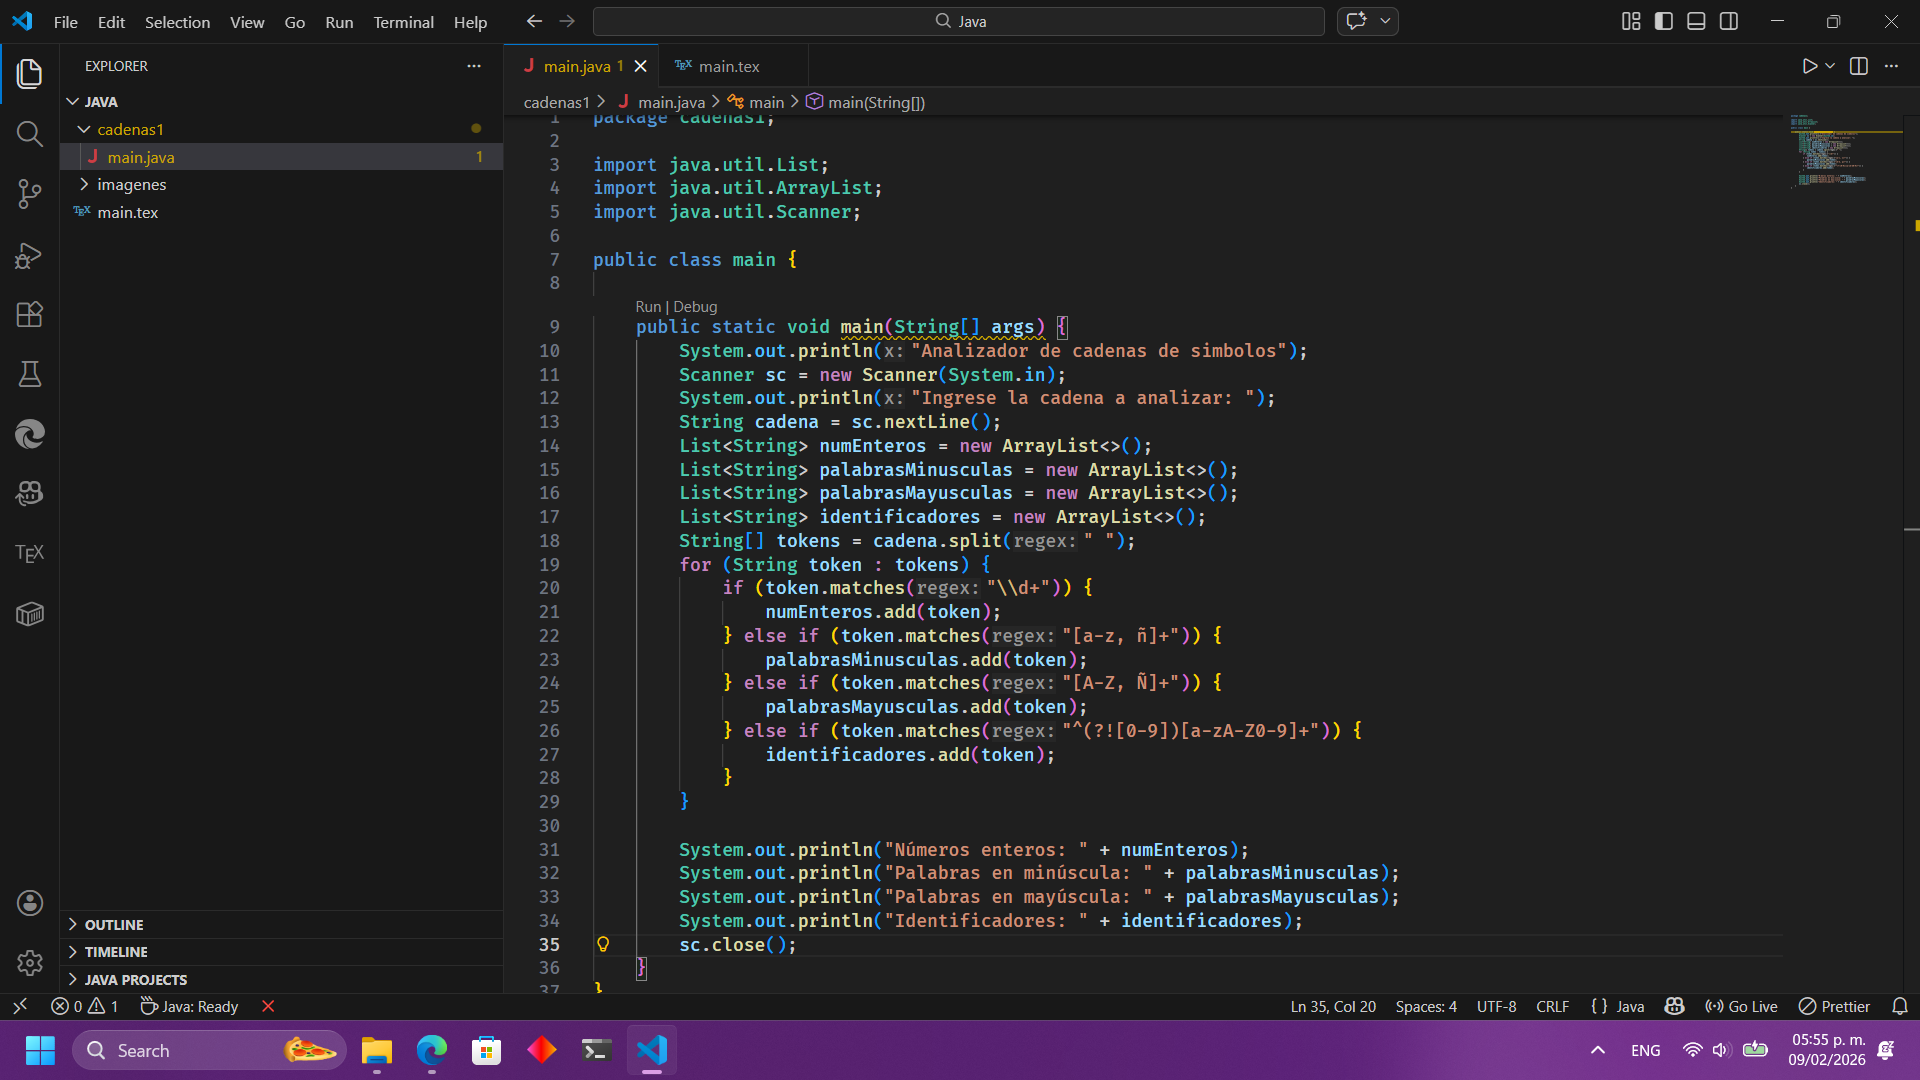
\includegraphics[width=15cm]{imagenes/programa.png}
    \newpage

\section{4. Cuestionario}
 ¿Cual es la utilidad de las expresiones regulares en la identificación de palabras de un lenguajes?  

 \texttt{Son de buen uso para la creación de patrones que resulten en una
 identificación de datos para verificar si un dato es valido o no}

 
 ¿Cuáles elementos del lenguaje de programación utilizaste para la implementación de las estructuras 
de datos?, ¿Cómo las utilizaste?
\texttt{Se uso el metodo splits() y el metodo matches() en java, se
utilizaron con el token y como una funcion junto con su expresion
regular}



 ¿Cuál es el proceso que seguiste para analizar las cadenas de símbolos? 

\texttt{1. Verificar que simbolos son, 2. Revisar que fila de caracteres se usara, 3. Crear una expresion regular simbolica con una pagina web, 4. Copiar y verificar la expresion con nuevos simbolos}
 
 ¿Qué elementos del lenguaje de programación te permitieron implementar expresiones reguales? 
\texttt{Las cadenas de caracteres (string) ya tienen varias funciones para
separar y modificarlas segun una expresion regular}
 
 ¿Qué condiciones o recomendaciones se deben seguir al escribir las expresiones regulares?
 \texttt{Usar correctamente los simbolos especiales, como ? (
 para opcional), + (para una cadena infinita), etc }
   
    
\section{5. Conclusiones}
   Con el programa se fortaleció el conocimiento de expresiones regulares
   las cuales son necesarias para frontends en paginas web, aplicaciones
   u otro tipo de datos que necesite un formato especifico, especialmente datos que puedan romper el programa
    
    \newpage
    
\section{Referencias Bibliográficas}
    %Formato APA 7° Ed.
    \begin{thebibliography}{100}
        \bibitem{regEx1}
TecnoDigital ({\bf 2025, 10 febrero}). Expresiones regulares (RegEx): Guía completa y ejemplos. Informática y Tecnología Digital.
 {\em https://informatecdigital.com/expresiones-regulares-regex/}

         \bibitem{regEx1}
Expresiones Regulares en Java: Guía Completa para su Uso. ({\bf 2025, 16 julio}). 4Geeks
 {\em https://4geeks.com/es/lesson/expresiones-regulares-java}
    \end{thebibliography}

\end{document}
